\documentclass[Royal,times,sageh]{sagej}

\usepackage{moreverb,url,natbib, multirow, tabularx}
\usepackage[colorlinks,bookmarksopen,bookmarksnumbered,citecolor=red,urlcolor=red]{hyperref}





\begin{document}

\title{Missing the Point\(\colon\) Non-Convergence in Iterative Imputation
Procedures}

\runninghead{Oberman}

\author{H. I. Oberman\affilnum{1}}

\affiliation{\affilnum{1}{Department of Methodology and Statistics, Utrecht University, Utrecht,
The Netherlands}}

\corrauth{Hanne Oberman, Sjoerd Groenman building, Utrecht Science Park, Utrecht,
The Netherlands.}

\email{\href{mailto:h.i.oberman@uu.nl}{\nolinkurl{h.i.oberman@uu.nl}}}

\begin{abstract}
(\textbf{Rewrite:}) Multple imputation by chained equations (mice) is a
widely used tool to accommodate missing data. While empirical evidence
supports the validity of inferences obtained using mice, there is no
consensus on the convergence properties of the method. This paper
provides insight into non-convergence of mice algorithms.
\end{abstract}

\keywords{MICE; convergence}

\maketitle

\hypertarget{introduction}{%
\section{Introduction}\label{introduction}}

Missing data problems are ubiquitous and pervasive in the social and
behavioral sciences. If a dataset contains just one missing value for a
variable of interest, statistical inferences are undefined and will not
yield results. Incomplete observations are therefore ignored by default
in many statistical packages (i.e., list-wise deletion is employed).
Unfortunaltely, this \emph{ad hoc} solution may yield wildly invalid
results \citep{buur18}. An alternative is to `impute' (i.e., fill in)
every missing value in the incomplete dataset. With imputation
techniques, one or several completed datasets are created, on which
statistical inferences can be performed. The case with several completed
datasets is known as `multiple imputation' \citep[MI;][]{rubin76}, and
requires and additional step to pool the results accross imputations.
Because this pooled result will reflect the uncertainty in the data due
to missingness, it is in many cases an unbiased and confidence valid
estimate of the true (but missing) data inference \citep{buur18}. A
popular method to obtain imputations is to use the `Multiple Imputation
by Chained Equations' algorithm, shorthand `MICE'. MICE is an iterative
algorithmic procedure to draw imputations from the posterior predictive
distribution of the missing values. This introduces a potential threat
to the validity of the imputations: what if the algorithm has not
converged? Are the implications then to be trusted? And can we rely on
the inference obtained on the completed data? These are open questions,
because the convergence of iterative imputation algortihms has not been
systematically studied \citep{buur18}. In this paper, we investigate the
convergence properties of iterative imputation procedures by means of
model based simulation in \texttt{R} list(title = ``R: A Language and
Environment for Statistical Computing'', author = list(list(given = ``R
Core Team'', family = NULL, role = NULL, email = NULL, comment = NULL)),
organization = ``R Foundation for Statistical Computing'', address =
``Vienna, Austria'', year = ``2020'', url =
``\url{https://www.R-project.org/}'').

Rubin's rules \citeyearpar{rubin76} may be used to reflect the
uncertainty in the inferences due to missingness by pooling the results
across `imputations'. A popular method to obtain imputations
completions, the analysis of scientific interest can be performed. It
has been , or to complete these observations by imputing the missing
values. Imputation is the method of filling in

by which That is, unless ad hoc solutions are employed (e.g., list-wise
deletion), which can yield invalid results. contains missing values,
statistical analyses cannot be performed without only be performed a
dataset contains missing values, statistical analyses can statistical
inferences cannot be performed\\
Missingness is problematic because statistical inference cannot be
performed on the whole data without employing \emph{ad hoc} solutions
(e.g., list-wise deletion), which may yield wildly invalid results
\citep{buur18}. A popular method to obtain statistically valid results
despite of missing data is `multiple imputation' \citep[MI;][]{rubin76}.
The multiple imputation method can be roughly divided into 3 steps:
First, each missing value in an incomplete dataset is `imputed' (i.e.,
filled in) several times by some algorithmic procedure. Next, the
analysis of scientific interest is performed on each of the completed
datasets. And finally, the results of these analyses are pooled into a
single aggregated statistic.

Algorithms are often used to draw imputations from the posterior
predictive distribution of the missing values. This introduces a
potential threat to the validity of the imputations: what if the
algorithm has not converged? Are the implications then to be trusted?
And can we rely on the inference obtained on the completed data?

There is no scientific consensus on the convergence properties of MI
algorithms \citep{taka17}. Some default techniques (e.g., `predictive
mean modeling') might not yield converged states at all \citep{murr18}.
Therefore, algorithmic convergence should be monitored carefully. The
current practice is visually inspecting imputation chains for signs of
non-convergence, but this may be challenging to the untrained eye
\citep[\(\S\) 6.5.2]{buur18}. Moreover, visually inspecting imputation
chains may only diagnose severely pathological cases of non-convergence.
Therefore, diagnostic evaluation of convergence would be preferred.

Iterative imputation algorithms such as mice, are MCMC methods, and
convergence of MCMC algorithms is not from a scalar to a point but from
one distribution to another. Therefore, generated values will vary even
after convergence. The aim of convergence diagnostics for MCMC methods
is thus not to establish the point at which convergence is reached, but
to diagnose severe non-convergence.

Several MCMC convergence diagnostics exist, but it is not known
whetherthese are appropriate for MICE. The application of convergence
diagnostics to MI methods has not been systematically studied
\citep{buur18}. The open questions are, e.g.: How can non-convergence be
diagnosed? How many iterations are sufficient/needed? What are the
effects of non-convergence on estimates, predictions and inference? What
is an appropriate non-convergence diagnostic? Are the default number of
iterations sufficient? The defaults of common MI software: SPSS = 10
\href{https://www.ibm.com/support/knowledgecenter/SSLVMB_24.0.0/spss/mva/syn_multiple_imputation_impute.html}{(link)},
Mplus = 100??
\href{https://pdfs.semanticscholar.org/e20e/29e008592cbfbaa567931f74cdfdb5451405.pdf?_ga=2.55354671.54033656.1584698748-527613517.1584698748}{(link)},
Stata = 10
\href{https://www.stata.com/manuals13/mi.pdf,\%20p.\%20139}{(link)},
Amelia = NA, because resampling, not convergence
\href{https://cran.r-project.org/web/packages/Amelia/Amelia.pdf}{(link)},
en MI = 30
\href{https://cran.r-project.org/web/packages/mi/mi.pdf}{(link)}.

For reasons of brevity, we only focus on the MI algorithm implemented in
the world-leading MI software: the \texttt{R} \citep{R} package
\texttt{mice} \citep{mice}. The convergence properties of this MI
algorithm are investigated through model-based simulation. The results
of this simulation study are guidelines for assessing convergence of MI
algorithms, which will aid applied researchers in drawing valid
inference from incomplete datasets.

\hypertarget{notation}{%
\subsection{Notation}\label{notation}}

Let \(y\) denote an \(n \times p\) matrix containing the data values on
\(p\) variables for all \(n\) units in a sample. The data value of unit
\(i\) (\(i = 1, \dots, n\)) on variable \(j\) (\(j = 1, \dots, p\)) may
be either observed or missing. The collection of observed data values in
\(y\) is denoted by \(y_{obs}\); the missing part of \(y\) is referred
to as \(y_{mis}\). (\textbf{This is not only notation, but theory too:}
For each datapoint in \(y_{mis}\), we sample \(M \times T\) times
plausible values, where \(M\) is the number of imputations
(\(m = 1, \dots, M\)) and \(T\) is the number of iterations
(\(t = 1, \dots, T\)).) The collection of samples between the initial
value (at \(t=1\)) and the final imputed value (at \(t=T\)) will be
referred to as an `imputation chain'.

\textbf{Add: missingness percentage = proportion of cases with one or
more missing values times 100 }

\hypertarget{convergence-diagnostics}{%
\section{Convergence diagnostics}\label{convergence-diagnostics}}

\textbf{(Start with current guidelines, then continue with possible
quant measures of the same things from MCMC lit.)} In iterative
algorithmic procedures (Markov chain Monte Carlo methods; e.g.,
\texttt{mice} algorithms or Gibbs samplers) non-convergence may be
present as non-stationarity within chains (i.e., trending), or as slow
mixing between chains (i.e., no intermingling (\textbf{source??})).
(\textbf{add example/guidelines visual inspection here?})

The stationarity component of convergence may be evaluated with
autocorrelation \citep[\(AC\);][]{scha97, gelm13}, numeric standard
error \citep[or `MC error';][]{gewe92}, and Raftery and Lewis's
\citeyearpar{raft91} procedure to determine the effect of trending
within chains (\textbf{or the chain length required to cancel out
trending?}).

The mixing component can be assessed with the potential scale reduction
factor \(\widehat{R}\) \citep[a.k.a. `Gelman-Rubin
statistic';][]{gelm92}. With an adapted version of \(\widehat{R}\),
proposed by \citet{veht19}, the stationarity component of convergence
might be evaluated as well. This would make \(\widehat{R}\) a general
convergence diagnostic. The application of \(\widehat{R}\) to assess
stationarity has not been thoroughly investigated. Therefore, this study
employs both \(\widehat{R}\) and autocorrelation to investigate
convergence, as recommended by \citep[p.~898]{cowl96}.

Note that all of these methods evaluate the convergence of univariate
scalar summaries (e.g., chain means or variances). These convergence
diagnostics cannot diagnose convergence of multivariable statistics
(i.e., relations between scalar summaries). \citet{buur18} proposed to
implement multivariable evaluation through eigenvalue decomposition
\citep{mack03}. This method is outside of the scope of the current study
(\textbf{not anymore?}).

\hypertarget{potential-scale-reduction-factor}{%
\subsection{Potential scale reduction
factor}\label{potential-scale-reduction-factor}}

To define \(\widehat{R}\), we follow notation by \citep[p.~5]{veht19}.
Let \(M\) be the total number of chains, \(T\) the number of iterations
per chain, and \(\theta\) the scalar summary of interest (e.g., chain
mean or chain variance). For each chain (\(m = 1, 2, \dots, M\)), we
estimate the variance of \(\theta\), and average these to obtain
within-chain variance \(W\).

\begin{align*}
W&=\frac{1}{M} \sum_{m=1}^{M} s_{j}^{2},  \text { where } s_{m}^{2}=\frac{1}{T-1} \sum_{t=1}^{T}\left(\theta^{(t m)}-\bar{\theta}^{(\cdot m)}\right)^{2}. 
\end{align*}

We then estimate between-chain variance \(B\) as the variance of the
collection of average \(\theta\) per chain.

\begin{align*}
B&=\frac{T}{M-1} \sum_{m=1}^{M}\left(\bar{\theta}^{(\cdot m)}-\bar{\theta}^{(\cdot \cdot)}\right)^{2}, \text { where } \bar{\theta}^{(\cdot m)}=\frac{1}{T} \sum_{t=1}^{T} \theta^{(t m)} \text{, } \bar{\theta}^{(\cdot \cdot)}=\frac{1}{M} \sum_{m=1}^{M} \bar{\theta}^{(\cdot m)}. 
\end{align*}

From the between- and within-chain variances we compute a weighted
average, \(\widehat{\operatorname{var}}^{+}\), which over-estimates the
total variance of \(\theta\). \(\widehat{R}\) is then obtained as a
ratio between the over-estimated total variance and the within-chain
variance:

\begin{equation*}
\widehat{R}=\sqrt{\frac{\widehat{\operatorname{var}}^{+}(\theta | y)}{W}},
\text{ where } \widehat{\operatorname{var}}^{+}(\theta | y)=\frac{N-1}{N} W+\frac{1}{N} B.
\end{equation*}

We can interpret \(\widehat{R}\) as potential scale reduction factor
since it indicates by how much the variance of \(\theta\) could be
shrunken down if an infinite number of iterations per chain would be run
\citep{gelm92}. This interpretation assumes that chains are
`over-dispersed' at \(t=1\), and reach convergence as \(T \to \infty\).
Over-dispersion implies that the initial values of the chains are `far
away' from the target distribution and each other. When all chains
sample independent of their initial values, the mixing component of
convergence is satisfied, and \(\widehat{R}\)-values will be close to
one. High \(\widehat{R}\)-values thus indicate non-convergence. The
conventionally acceptable threshold for convergence was
\(\widehat{R} < 1.2\) \citep{gelm92}. More recently, \citet{veht19}
proposed a more stringent threshold of \(\widehat{R} < 1.01\).

\hypertarget{autocorrelation}{%
\subsection{Autocorrelation}\label{autocorrelation}}

Following the same notation, we define autocorrelation as the
correlation between two subsequent \(\theta\)-values within the same
chain \citep[p.~147]{lync07}. In this study we only consider \(AC\) at
lag 1, i.e., the correlation between the \(t^{th}\) and \(t+1^{th}\)
iteration of the same chain.

\begin{equation*}
AC = \left( \frac{T}{T-1} \right) \frac{\sum_{t=1}^{T-1}(\theta_t - \bar{\theta}^{(\cdot m)})(\theta_{t+1} - \bar{\theta}^{(\cdot m)})}{\sum_{t=1}^{T}(\theta_t - \bar{\theta}^{(\cdot m)})^2}.
\end{equation*}

We can interpret \(AC\)-values as a measure of stationarity. If
\(AC\)-values are close to zero, there is no dependence between
subsequent samples within imputation chains. Positive \(AC\)-values,
however, indicate recurrence. If \(\theta\)-values of subsequent
iterations are similar, trending may occur. Negative \(AC\)-values show
no threat to the stationarity component of convergence. On the contrary
even---negative \(AC\)-values indicate that \(\theta\)-values of
subsequent iterations diverge from one-another, which may increase the
variance of \(\theta\) and speed up convergence. As convergence
diagnostic, the interest is therefore in positive \(AC\)-values.
Moreover, the magnitude of \(AC\)-values may be evaluated statistically,
but that is outside of this note's scope.

Negative \(AC\)-values indicate divergence within imputation chains.
Subsequent sampled values within each imputation chain are less alike.
It may not be wise (\textbf{why? and how would we know? e.g., wider
distrubutions? didn't seem like it\ldots{}}) to terminating the
algorithm when AC is negative. \textbf{High \(AC\)-values are
implausible in MI procedures. That is, the randomness induced by the MI
algorithm effectively mitigates the risk of dependency within chains.}

In short, convergence is reached when there is no dependency between
subsequent iterations of imputation chains (\(AC = 0\)), and chains
intermingle such that the only difference between the chains is caused
by the randomness induced by the algorithm (\(\widehat{R} = 1\)).

\hypertarget{simulation-hypothesis}{%
\subsection{Simulation Hypothesis}\label{simulation-hypothesis}}

This study evaluates whether \(\widehat{R}\) and \(AC\) could diagnose
convergence of multiple imputation algorithms. We assess the performance
of the two convergence diagnostics against the recommended evaluation
criteria for MI methods \citep[i.e., average bias, average confidence
interval width, and empirical coverage rate across simulations;][\(\S\)
2.5.2]{buur18}. That is, there is no baseline measure available to
evaluate performance against.

Based on an empirical finding \citep{lace07}, we hypothesize that
\(\widehat{R}\) will over-estimate non-convergence of MI algorithms. The
threshold of \(\widehat{R} < 1.01\) will then be too stringent for
diagnosing convergence. This over-estimation may, however, be diminished
because \(\widehat{R}\) can falsely diagnose convergence if initial
values of the algorithm are not appropriately over-dispersed
\citep[p.~437]{broo98}. In \texttt{mice}, initial values are chosen
randomly from the observed data. Therefore, we cannot be certain that
the initial values are over-dispersed. We expect this to have little
effect on the hypothesized performance of \(\widehat{R}\). \textbf{(Add
actual hypothesis.)} No hypothesis was formulated about the performance
of \(AC\) as convergence diagnostic.

\hypertarget{simulation-study}{%
\section{Simulation study}\label{simulation-study}}

The convergence of \texttt{mice} is investigated through model-based
simulation in \texttt{R} \citep[version 3.6.3;][]{R}. The simulation
set-up is summarized in the pseudo-code below. The complete \texttt{R}
script of the simulation study is available from
\href{https://github.com/gerkovink/shinyMice/tree/master/3.Thesis/1.SimulationStudy}{github.com/gerkovink/shinyMice}.

A finite population of \(N=1000\) is simulated to solve a multiple
linear regression problem, where dependent variable \(Y\) is regressed
on independent variables \(X_1\), \(X_2\) and \(X_3\) (\textbf{check
notation with betas here, and add what the quantity/-ies of scientific
interest is/are!}):

\[Y \sim \beta_1 X_1 + \beta_2 X_2 + \beta_3 X_3.\]

The data generating model is a multivariate normal distribution

\begin{align*}
\begin{pmatrix}X_1\\
X_2\\
X_3\\
\epsilon
\end{pmatrix} \sim  N
\begin{bmatrix}
\begin{pmatrix}
12\\
3\\
0.5\\
0
\end{pmatrix}\!\!,
\begin{pmatrix}
4 & 4 & 1.8 & 0\\
4 & 16 & 4.8 & 0\\
1.8 & 4.8 & 9 & 0\\
0 & 0 & 0 & 100
\end{pmatrix}
\end{bmatrix}\\[2\jot]
\end{align*}

Outcome variable \(Y\) is subsequently calculated as
\[Y =  1 + 2X_1 + .5X_2 - X_3 + \epsilon .\]

\textbf{Add the function \texttt{mvtnorm::rmvnorm()} back in} use
citation(``mvtnorm'')

The complete data is `amputed' once for each simulation repetition with
function \texttt{mice::ampute()}. (\textbf{change this:} The missingness
is univariate, and the probability to be missing is the same for all
four variables, namely 20\% (\texttt{prop\ =\ 0.8,\ mech\ =\ "MCAR"}).
This leaves 20\% of the rows completely observed). \textbf{(Add
different percentages missingness??)} This study only considers only an
MCAR missingness mechanism. Therefore, results may not be extrapolated
to other missing data problems. Proper performance of the convergence
diagnostics under MCAR is necessary but not sufficient to demonstrate
appropriateness of \(\widehat{R}\) and \(AC\) as convergence
diagnostics. This is just a proof of concept.

Missing datapoints are imputed with the function \texttt{mice::mice()}.
All MI procedures are performed with Bayesian linear regression
imputation (\texttt{method\ =\ "norm"}), and five imputation chains
(\texttt{m\ =\ 5}). The number of iterations varies between simulation
conditions (\texttt{maxit\ =} \(1, 2, \dots, 100\)).

\(\widehat{R}\) (\textbf{of what?? i.e., chain means and chain variances
of each variable}) is computed by implementing Vehtari et al.'s
\citeyearpar{veht19} recommendations. \(AC\) (\textbf{of what? and how
is AC aggregated across imputations? i.e., mean in latest sim}) is
computed with function \texttt{stats::acf()}.

To estimate the quantity of scientific interest, \(Q\), we perform
multiple linear regression on each completed dataset with the function
\texttt{stats::lm()}. We obtain an estimated regression coefficient per
imputation, which are pooled into a single estimate, \(\bar{Q}\). We use
the function \texttt{mice::pool()} to estimate u bar (\textbf{check wat
dat nou precies is!!}) according to Rubin's \citeyearpar{rubin87} rules,
and subsequently implement finite population pooling conform
\citet{vink14}.

We compute bias as the difference between \(Q\) and \(\bar{Q}\).
Confidence interval width (CIW) is defined as the difference between the
lower and upper bound of the 95\% confidence interval (CI95\%) around
\(\bar{Q}\). We compute the CI95\% bounds as

\[\bar{Q} \pm t_{(m-1)} \times SE_{\bar{Q}},\]

where \(t_{(m-1)}\) is the quantile of a \(t\)-distribution with \(m-1\)
degrees of freedom, and \(SE_{\bar{Q}}\) is the square root of the
pooled variance estimate. \textbf{Why track CIW?} Under-estimating the
variance of \(\bar{Q}\) may yield spurious inferences. From bias and
CIW, we calculate empirical coverage rates. Coverage rate is the
proportion of simulations in which \(Q\) is between the bounds of the
CI95\% around \(\bar{Q}\).

\hypertarget{results}{%
\section{Results}\label{results}}

\textbf{(Add more info about figure legends and axes.)}

\hypertarget{univariate-estimates-and-convergence-diagnostics-theta-mean-and-theta-variance}{%
\subsection{Univariate estimates and convergence diagnostics (theta =
mean and theta =
variance)}\label{univariate-estimates-and-convergence-diagnostics-theta-mean-and-theta-variance}}

The bias in the estimates of the variable means show little to no
difference between simulation conditions. It doesn't seem to matter how
many iterations you use in the mice algorithm, the estimates are
unbiased. Similarly, the bias in the estimated variances is more or less
stable across simulation conditions. These univariate quantities appear
to be unaffected by the number of iterations.

When applied to the imputation chain means, \(\widehat{R}\) indicates
that the mice algorithm does not reach a converged state
(\(\widehat{R}\) = 1) in any of the simulation conditions. Neither is
the most recent recommended threshold reached (\(\widehat{R}\)
\textless{} 1.01). The conventional \(\widehat{R}\) threshold of 1.2 is
reached in simulation conditions \(T = 3\) and \(T > 6\). (With the
default number of iterations (maxit = 5), this dip in Rhat values would
be spotted, so it is no problem.) The point at which an extra iteration
does not seem to improve the Rhat value is around \(T=30\).

Auto-correlations indicate no sign of trending within imputation chains.
In most simulation conditions AC is smaller than or about equal to zero.
Across simulation conditions, however, the autocorrelation curve does
not trend towards 0. Autocorrelation values plateau off at a value of
around .1 . This is a small positive autocorrelation, which would
indicate some trending within chains.

The \(\widehat{R}\) and \(AC\) values for the imputation chain variances
show equal trends and are therefore not discussed separately. Taken
together, univariate estimates seem robust across simulation conditions.
There is no clear effect of the number of iterations on the bias in
these estimates, while the convergence diagnostics indicate that the
algorithm did not reach a completely converged state (yet).

\hypertarget{multivariate-estimates}{%
\subsection{Multivariate estimates}\label{multivariate-estimates}}

There is a clear bias in the regression estimates in simulation
conditions where the number of iterations is smaller than four. In
simulation conditions where \(T > 5\) there is little to no bias in the
estimated regression coefficients. In most simulation conditions nominal
coverage is obtained (i.e., coverage rates of .95) for the confidence
intervals around the regression coefficients. Conditions with only one
or two iterations show some undercoverage. Since confidence interval
width is stable across conditions, the undercoverage may be attributed
to the bias in the estimated regression coefficients.

If we look at the estimated proportion of explained variance in outcome
variable Y we see that the coefficient of determination is underestimate
estimated in conditions where the number of iterations is equal to two
or less, and slightly overestimated in conditions where the number of
iterations is equal to three or more.

In short, we see that the minimum number of iterations required to
obtain unbiased, confidence valid regression estimates is 5. This value,
however, is dependent on the percentage of missing values. E.g., with
95\% of cases having missing data we need at least seven iterations to
obtain unbiased results.

\begin{flushleft}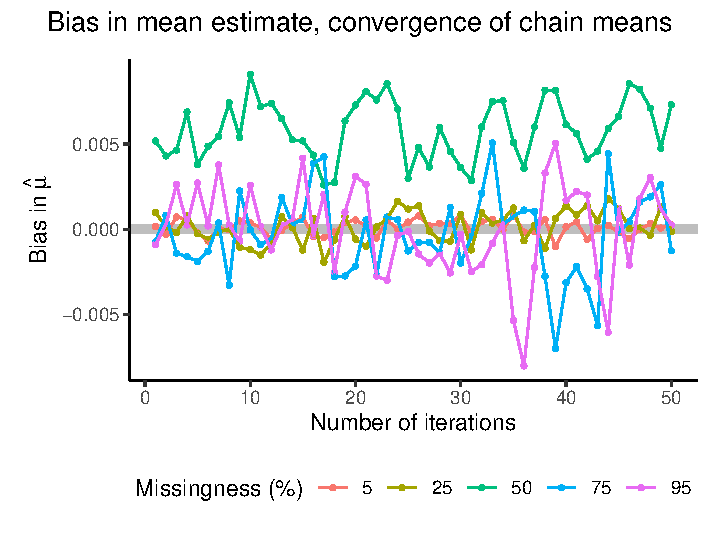
\includegraphics{manuscript_files/figure-latex/unnamed-chunk-3-1} \end{flushleft}

\hypertarget{results-old-just-for-reference}{%
\section{Results {[}OLD, JUST FOR
REFERENCE!{]}}\label{results-old-just-for-reference}}

\hypertarget{convergence-diagnostics-1}{%
\subsection{Convergence Diagnostics}\label{convergence-diagnostics-1}}

\textbf{(Pair convergnce diagnostics with respective estimates, not
split between convergence and simulation diagnostics)}

It is apparent that there is a relation between the number of iterations
per simulation condition (\(T\)) and the convergence diagnostics.
Generally speaking, conditions with longer imputation chains (higher
\(T\)) coincide with less signs of non-convergence
(\(\widehat{R}\)-values approach one, and \(AC\)-values approach zero).

Figure 2A shows that \(\widehat{R}\)-values generally decrease with
increasing imputation chain lengths. The decline stabilizes somewhere
between the simulation conditions \(T=30\) and \(T=50\). The downward
trend is most pronounced for \(T=3\), and between \(T = 5\) and
\(T = 10\). In the intervening conditions (\(3 \leq T \leq 5\)),
however, we observe a steep increase in \(\widehat{R}\)-values. This
increase implies that non-convergence is under-estimated, and
convergence should not be diagnosed at this point (\textbf{is that
true???}). Based on the conventional threshold \(\widehat{R} < 1.2\), we
would falsely diagnose convergence at \(T=3\). According to the widely
used threshold \(\widehat{R} < 1.1\), convergence would be diagnosed for
conditions where \(T>9\). If we use the recently recommended threshold
\(\widehat{R} < 1.01\), we would conclude that convergence is reached in
none of the simulation conditions.

The \(AC\)-values displayed in Figure 2B are almost uniformly increasing
as a function of \(T\). The only \(AC\)-value that deviates from this
observation is for \(T=2\). The lowest \(AC\)-value is obtained for
\(T=3\). \%At \(T=5\), the \(AC\)-value reaches the level observed at
\(T=2\). The gradual increase plateaus between \(T=10\) and \(T=30\).
\(AC\)-values in conditions where \(T>70\) are indifferentiable from
zero, indicating stationarity. We see an initial decrease between
\(T=2\) and \(T=3\). Simulation conditions where \(T>5\) have
\(AC\)-values greater than \(T=2\) (\textbf{weird wording}).

According to this diagnostic, none of the simulation conditions show
signs of non-convergence, since we only observe negative or zero
\(AC\)-values.

Taken together, we see that \(T>3\) is the minimal requirement to
diagnose convergence (\(\widehat{R} < 1.2; AC \leq 0\)). This threshold
is, however, not sufficient, since we overlook the increase in
\(\widehat{R}\)-values up-to conditions where \(T>5\), and the
convergence diagnostics only reach stability at \(T>20\).

\hypertarget{simulation-diagnostics}{%
\subsection{Simulation Diagnostics}\label{simulation-diagnostics}}

We use average bias, average confidence interval width, and coverage
rate as performance measures to evaluate \(\widehat{R}\) and \(AC\)
(\textbf{not the goal! we want to show the effects of non-conv, not just
see how to diagnose it.}). We make the general observation that the
simulation diagnostics behave as theorized for most simulation
conditions (bias around zero, stable confidence interval widths, nominal
coverage rate at 95\%).

Figure 3A shows that bias is fairly stable across simulation conditions.
The condition \(T=1\) clearly deviates from this trend with a negative
bias. The bias for \(T=2\) is below average, but within the range of
fluctuations. Conditions where \(T>3\) can be diagnosed as unbiased, but
the average bias across iterations (as shown by a flat Loess line) only
reaches stability at \(T=20\) (\textbf{Loess might not be relevant,
check and remove accordingly!}).

CIW is only clearly divergent in the simulation condition \(T=1\), see
Figure 3B. Only conditions where \(T>3\) are therefore considered
sufficient. (\textbf{Possibly irrelevant Loess:} These conditions have
similar CIWs, but across iterations stability is not established (i.e.,
the Loess line is never completely flat within the 100 simulation
conditions).)

The empirical coverage rate across repetitions seems more or less stable
for conditions where \(T>1\), see Figure 3C. We see some over-coverage
at \(T=2\), but that is better than under-estimating the variance of
\(\bar{Q}\). On average, the coverage rate is somewhat higher than the
expected nominal coverage of 95\% \citep{neym34} (\textbf{not
anymore??}). (\textbf{Loess:} Similar to the CIWs, there is some
trending across iterations (i.e., the Loess line is never flat)).

From the simulation diagnostics, we observe that unbiased estimates with
nominal coverage rates were obtained in conditions where \(T>3\). This
suggests that as little as four iterations may be sufficient for the MI
algorithm under the current circumstances.

In short, there is a discrepancy between what the convergence
diagnostics and what the performance measures indicate. While \(T=4\)
seems sufficient with respect to simulation quantities, the condition
where \(T=4\) resulted in the `one-but-worst' values of both convergence
diagnostics. Complete algorithmic convergence as indicated by
\(\widehat{R}\) and autocorrelation is not reached in conditions where
\(T<20\).

\hypertarget{discussion}{%
\section{Discussion}\label{discussion}}

This note shows that convergence diagnostics \(\widehat{R}\) and \(AC\)
may diagnose convergence of multiple imputation algorithms, but their
performance differs from conventional applications to iterative
algorithmic procedures. (\textbf{nope! it shows that MICE can lead to
correct outcomes when they have not converged accroding to two common
conv diags. This may be due to the measures (e.g., assumption of
overdisp) or due to the Qs (lm reg coeff, not higher dimensional/more
complex RQs). Add what \%miss has to do with it.})\\
\(\widehat{R}\) and autocorrelation indicate that algorithmic
convergence may only be reached after twenty or even forty iterations,
while unbiased, confidence valid estimates estimates may be obtained
with as little as four iterations. These results are in agreement with
the simulation hypothesis: \(\widehat{R}\) over-estimates the severity
of non-convergence when applied to MI procedures. \%This may be due to
the quantity of scientific interest chosen. More `complicated' \(Q\)s
(e.g., higher order effects or variance components) might show bias,
under- or over-coverage at higher \(T\).

According to this simulation study, the recently proposed threshold of
\(\widehat{R}<1.01\) may be too stringent for MI algorithms.
(\textbf{This is only one of the goals: to give applied researchers a
diagnostic to indicate that they should keep iterating. The other is the
default in mice and other software packages, and yet another is \ldots{}
i forgot}) Under the relatively easy missing data problem of the current
study, the threshold was not reached. The other extreme of the
\(\widehat{R}\)-thresholds, the conventionally acceptable
\(\widehat{R} <1.2\), may be too lenient for MI procedures. Applying
this threshold to the current data, lead to falsely diagnosing
convergence at \(T = 3\) (\textbf{because it goes up after, not because
it is not converged enough}). It appears that the widely used threshold
of \(\widehat{R} < 1.1\) suits MI algorithms the best. We might,
however, also formulate a new threshold, specifically for the evaluation
of MI algorithms. The current study suggests that \(\widehat{R} < 1.05\)
may be implemented, since that is the level at which the \(\widehat{R}\)
stabilize (around \(T = 20\)) (\textbf{Not necessary for this Q, but
maybe for more complicated Qs}).

The negative \(AC\)-values obtained in this study show no threat of
non-stationarity. However, initial dip in \(AC\)-values may have
implications for the default number of iterations in \texttt{mice}
(\texttt{maxit\ =\ 5}). Terminating the algorithm at \(T=5\) may not be
the most appropriate, since this lead to the worst convergence
(\textbf{nope, only for Rh, not AC}), as indicated by \(\widehat{R}\)
and \(AC\). Under the current specifications, \(T>20\) would be more
appropriate.

The observed dip in AC implies that default maxit value of five
iterations is the worst possible number of iterations. Moreover, the
results of this study imply that assessing the stationarity component of
convergence with \(AC\) might be redundant.

Further research is needed to investigate their performance under clear
violation of convergence, e.g.~dependency between predictors (predictors
with very high correlations). Until then, we have only shown that the
convergence diagnostics can diagnose non-convergence of MI algorithms
that trend towards a converged state. Also for future research, look at
developing a convergence diagnostic for substantive models, and
implement a Wald test for \(AC = 0\).

\bibliographystyle{sageh}
\bibliography{thesis.bib}


\end{document}
